\section{Problem statement}

In this assignment the core functionality which is exposed is
\emph{parsing} such a 32-bit number representing an instruction from
the MIPS32-instruction set and outputting other representations of the
same instruction, as well as some additional information regarding the
very same instruction, see Fig. \ref{fig:mips32-decompiler}.

\begin{figure}[H]
  \centering
  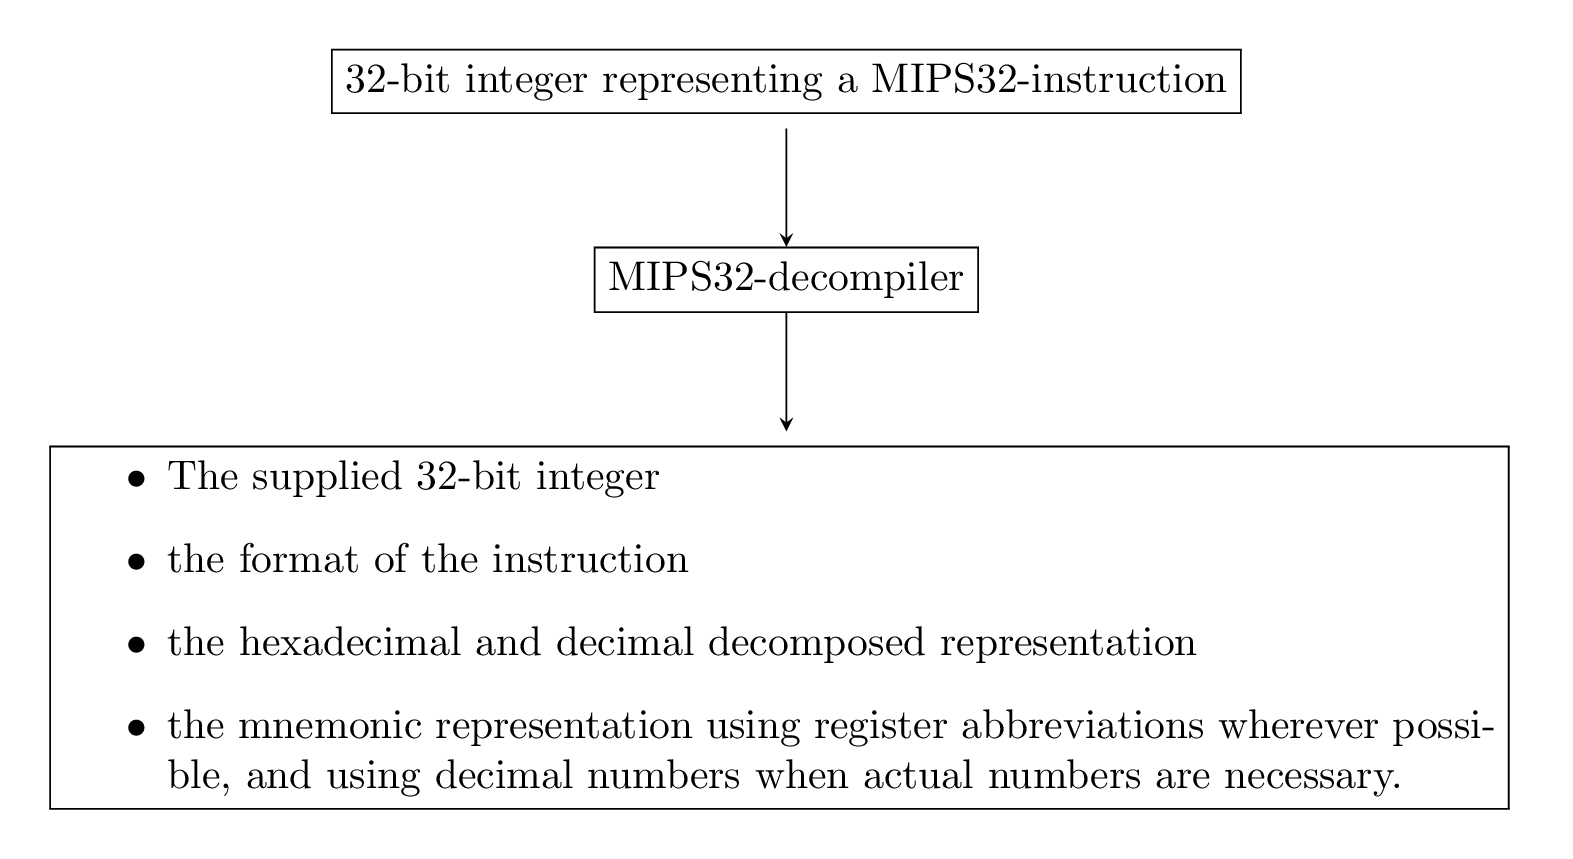
\includegraphics[width=0.9\textwidth]{figures/mips32-decompiler.png}
  \caption{Input and output of the decompiler}
  \label{fig:mips32-decompiler}
\end{figure}

Therefore, we need to be able to identify the appropriate format (from
which we can infer the decomposition), the identity of the particular
instruction (so that we can get its name) and also interpret the
constituent bitfields of the instruction so that we output a mnemonic
representation of the instruction.

In the previous section we established the terminology we will use
throughout the document. This terminology will also be used to
decompose our system that solves the problem at hand, viz. that
we will model our solution according to the problem domain.

Specifically, we will create a system such that when we take in a
32-bit integer representing a valid or semi-valid MIPS32-instruction
then we can construct an object instance named \mij{Instruction} that
knows, or can retrieve information about,\footnote{Using its
collaborators}

\begin{table}
\begin{itemize}
\item Its numerical representation
\item Its own format
\item Its own decomposed representation presented in both:
\subitem Hexadecimal form
\subitem Decimal form
\item Its own mnemonic representation
\end{itemize}
\caption{\mij{Instruction} operations/fields}
\label{table:instruction-operations}
\end{table}

The \mij{Instruction} class is an abstraction providing an
encapsulation around the aforementioned points. Ultimately, the system
will be divided into the self-explanatory constituents

\begin{itemize}
\item \formatm: R, I, J
\item \opcodem: An abstraction around the numerical opcode.
\item \formatm: Can for a given \opcodem return the associated format.
\item \decomposedm: Can decompose a 32-bit number into varying lengths.
\item \registerm: Associates a number with the register name, 
      see Table.~\ref{table:mips-register-naming-convention}
\end{itemize}

The \emph{core} issues to address is that of identifying the
instruction, validating the values of the bitfields of the
instruction, and outputting it according to some \emph{pattern}.

We will now address these issues in more detail, and create a running
tally of functionality that we would like to express within our
system. Afterwards we will define a fascimilie of a domain-specific
language (DSL) that will encode the items we touch upon here.

\subsection{Identifying the instruction}\label{section:identification}

Recall from our earlier example where we decompiled a \tt{mul}
instruction that the \opcode is always sufficient to identify
the format of the instruction it is not always sufficent to
identify an instruction uniquely.

We find that all J-type instructions and for some, but not all, I-type
instructions the \opcode will suffice. Specifically, those I-type
instructions which cannot be identified by their opcode alone is the
branch instructions and immediate trap operations.

For the opcodes \tt{op=0x00}, and \tt{op=0x1c} it is necessary to
consult a second field in order to identify the instruction
completely, namely the \tt{funct} field. For instructions with the
opcode \tt{0x01} the \tt{rt} field must instead be consulted.

Therefore, we would like to compose a system that may

\begin{itemize}
\item Get the six left-most bits from a 32-bit integer, i.e. the numerical opcode.
\item Infer the Format from the opcode.
\item When necessary consult additional bitfields in the 32-bit integer to
      determine the particular instruction.
\end{itemize}

\subsection{Validating the non-identifying bitfields}\label{section:validation}

Consider the 32-bit integer \tt{0x00012122}. This number represents an
instance of the \tt{sub} instruction. It is identified by
having its opcode set to \tt{0x00} and its funct field to \tt{0x22}.
\emph{But}, it is not \emph{valid} if its shamt field is not also set to 0.

This validation step needs to be incorporated somehow. It would be
naive to consider this an additional consultation of a bitfield to
determine identity, since we could not distinguish between whether or
not the correct instruction has been identified or if there is a
problem in the validation.

Hence, our system should be able to (once the particular instruction
has been identified) validate the instruction.

\subsection{Patternizing output}\label{section:patternizing}

We have not addressed this before but the mnemonic representation of
instructions in the MIPS32 instruction set has a tendency to follow a
certain pattern, and these patterns are dependent upon the format of
the particular instruction.

For an example, the instructions

\begin{verbatim}
add, addu, sub, mul, and, or, nor, xor, movn, movz
\end{verbatim}

\newcommand{\pattern}[1]{\emph{$\langle$#1$\rangle$}}
among possibly others, have the common pattern \pattern{iname, rd, rs,
rt} with \emph{iname} being the name of the instruction.

Other common patterns include 

\begin{itemize}
\item \pattern{iname rd, rs}
\item \pattern{iname rd, rt, rs}
\item \pattern{iname, rd, rt, shamt}
\end{itemize}

for R-format instructions and

\begin{itemize}
\item \pattern{iname, rt, rs, imm}
\item \pattern{iname rt, imm}
\item \pattern{iname, rt, rs(addr)}
\end{itemize}

for I-format instructions.

Being a RISC architecture we would expect these patterns to favor
regularity, and that maybe the above set would suffice but there
are in fact numerous others.

As such we will want to, for each instruction, associate it with its
output pattern.
